\begin{figure}
\centering
\subfigure[Late Fusion with Linear Interpolation]{
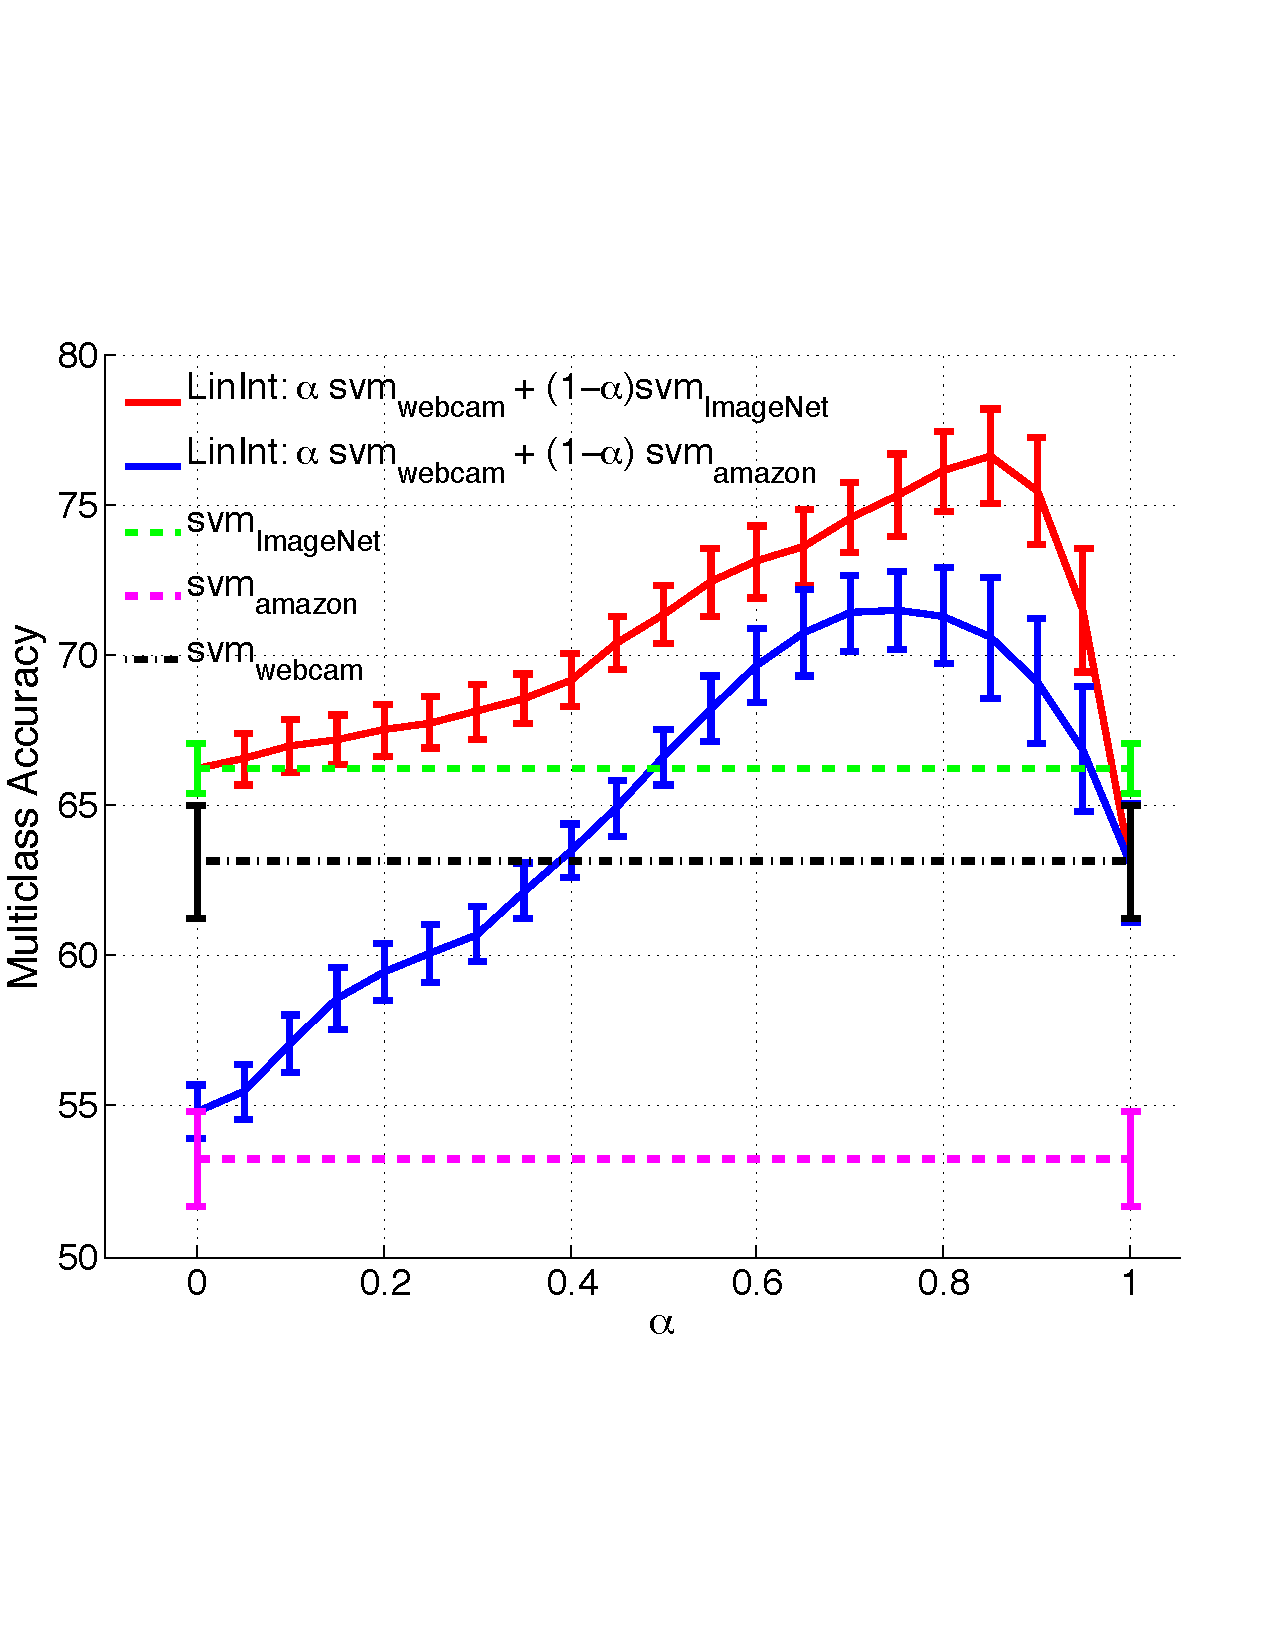
\includegraphics[height=.25\linewidth]{figs/amazonAndImagenet-linint-vs-alpha_C1_fc8.pdf}
\label{fig:linint-eval}
}
\subfigure[Unsupervised Methods]{
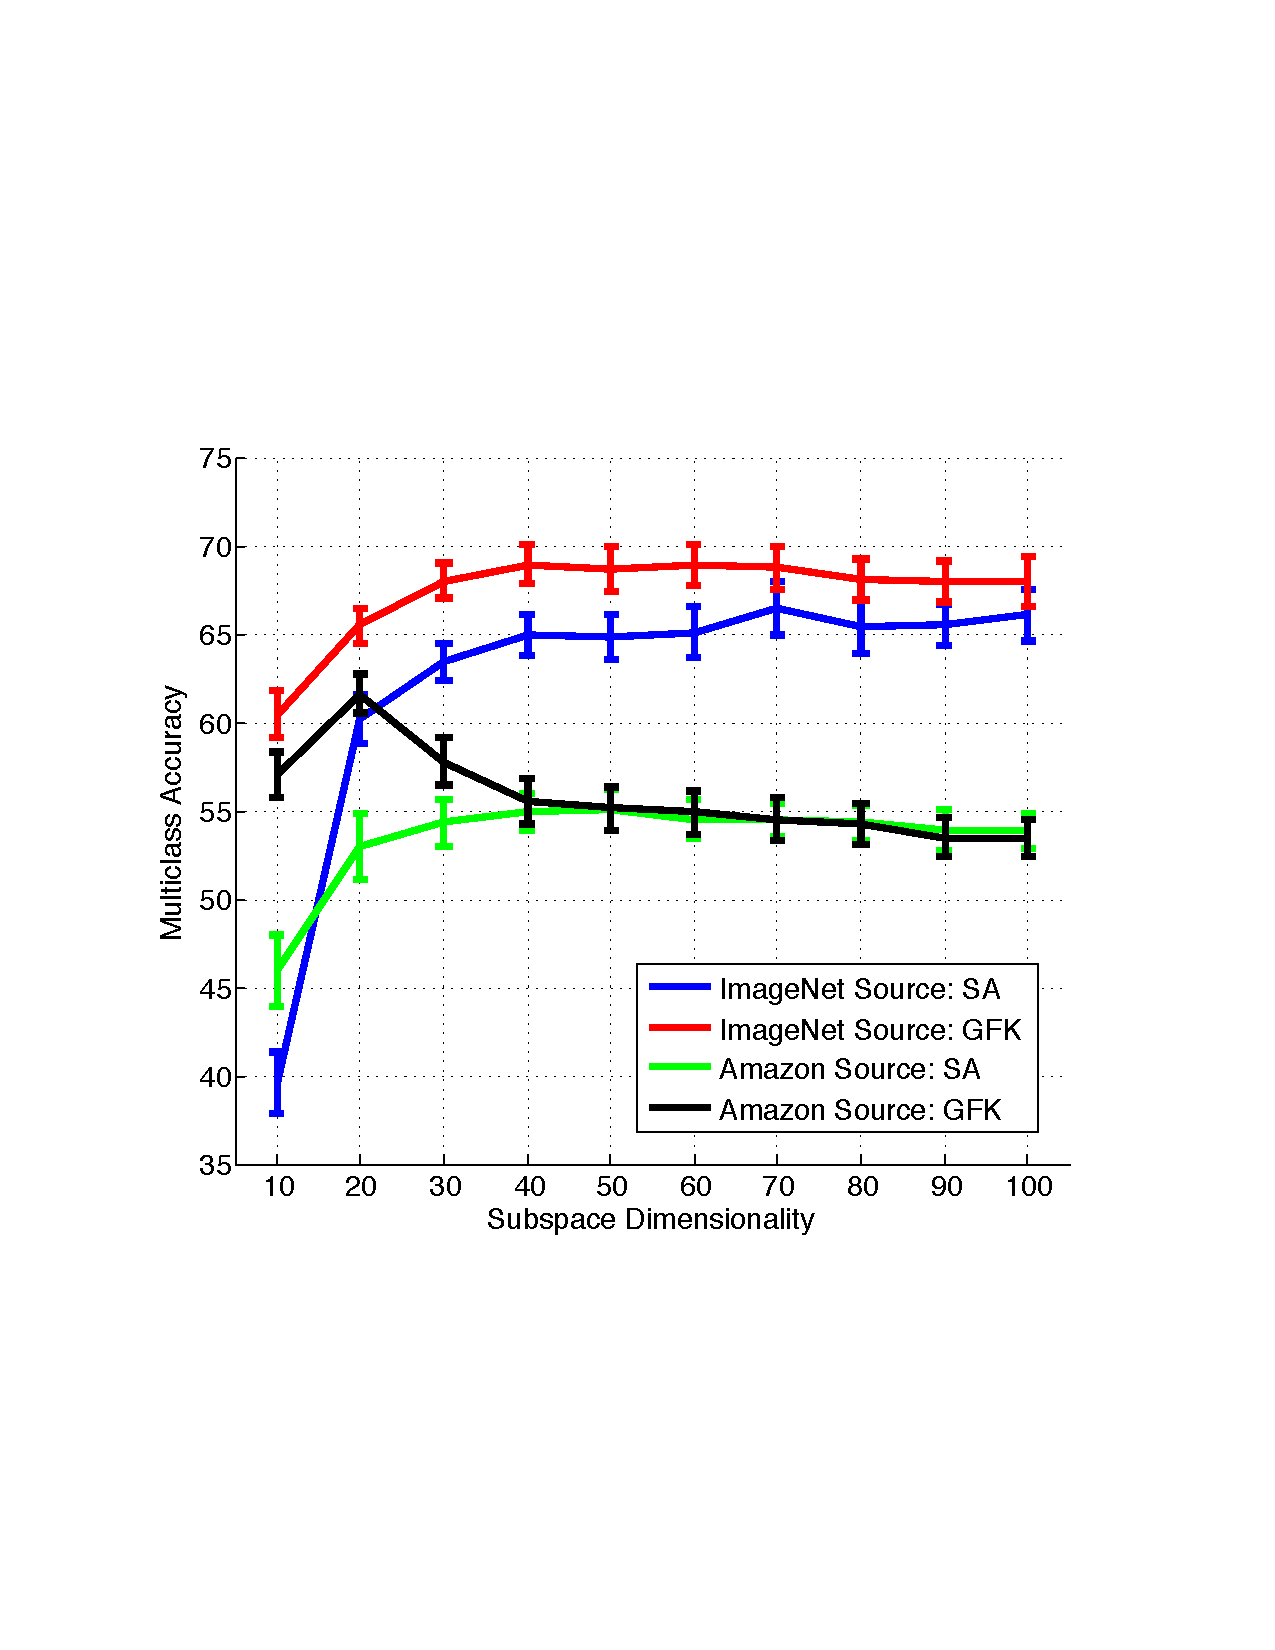
\includegraphics[height=.25\linewidth]{figs/amazonAndImagenet-sa_gfk_dim_C1_fc7.pdf}
\label{fig:sagfk-eval}
}
\subfigure[Feature Representation]{
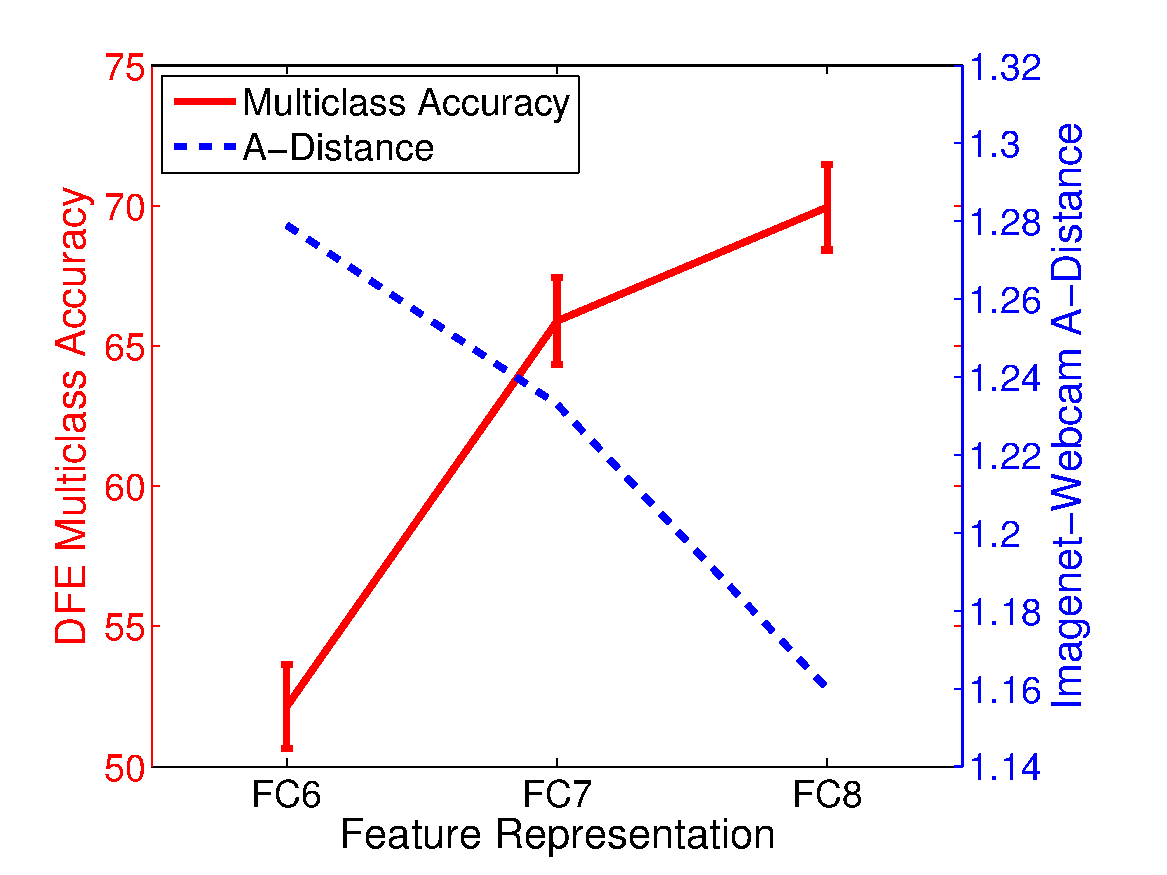
\includegraphics[height=.25\linewidth]{figs/imgnet_webcam_a_dist}
\label{fig:a-dist-eval}
}
\caption{Evaluation of hyperparameters for domain adaptation methods. (a) Analysis of the combination hyperparameter $\alpha$ for Deep Late Fusion (DLF) with linear interpolation: We find that choosing to weight the target domain higher than the source domain performs best.  (b) Analysis of the subspace dimensionality for Deep Subspace Alignment (DSA): The algorithm is not sensitive to the subspace dimension chosen. (c) Analysis of model selection: after which pre-trained layer do we add our adaptation layer: We show that using our layer selection criteria (A-distance) correlates with final classification accuracy.}
\label{fig:hyperparam-eval}
\end{figure}
